\documentclass[]{article}
\usepackage{listings}
\usepackage{xcolor}
\usepackage{amssymb}
\usepackage{hyperref}
\usepackage{tikz}
\usepackage{pgfplots}
\usepackage{multirow}
%opening
\title{CSC373 Week 6 Tutorial}
\author{}

\begin{document}

\maketitle

%\section{Midterm Review}
%Go over questions 5 and 6 on the midterm.

\section{\href{https://web.stanford.edu/class/archive/cs/cs161/cs161.1138/lectures/18/Small18.pdf}{Bellman-Ford}}
The Bellman-Ford algorithm can be used to find the shortest path tree from a single vertex. It is similar to Dijkstra's algorithm, in that regard, but it works on graphs with negative edges. Negative cycles, if found, cause the program to terminate since they create infinite loops.
%\textit{ Set the distance to each node to be infinity except the source, set to 0. Iterate over the following relaxation $n$ times (since the longest path has, at most, n edges). To relax a vertex, check if the distance to that vertex can be reduced by setting a new parent. If so, reduce the cost to that vertex and save the new parent.}

\begin{itemize}
	\item Trace how Dijkstra's algorithm runs on the graph below to see how it fails.
	\item Bonus: Trace how Bellman-Ford runs and try to find ways to improve it.
\end{itemize}

\begin{figure}
	\centering
	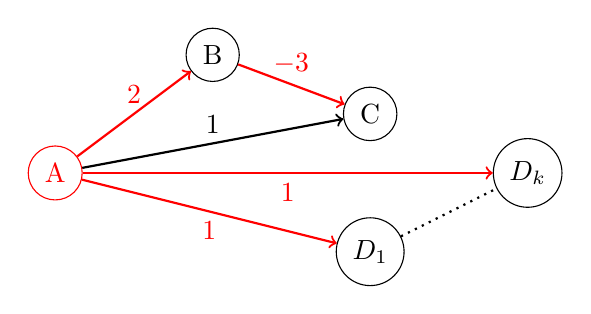
\begin{tikzpicture}
	\node[draw,circle,color=red] (A) at (0,-1.5) {A};
	\node[draw,circle] (B) at (2,0) {B};
	\node[draw,circle] (C) at (4,-.75) {C};
	\node[draw,circle] (Dk) at (6,-1.5) {$D_k$};
	\node[draw,circle] (D1) at (4,-2.5) {$D_1$};
	
	\draw [->, thick, color=red] (A) edge node[above] {$2$} (B);
	\draw [->, thick] (A) edge node[above] {$1$} (C);
	\draw [->, thick, color=red] (B) edge node[above] {$-3$} (C);
	
	\draw [->, thick, color=red] (A) edge node[below] {$1$} (D1);
	\draw [->, thick, color=red] (A) edge node[below] {$1$} (Dk);
	\draw [dotted, thick] (D1) edge node[below] {} (Dk);
	
	
	\end{tikzpicture}
	\caption{Graph with k-claw from $a$ to $D_i, 1 \leq i \leq k$. Shortest path tree from source $A$ is highlighted red}
\end{figure}
If we get this far, the answer is \href{https://wcipeg.com/wiki/Shortest_Path_Faster_Algorithm}{Shortest Path Faster Algorithm (SPFA) aka Yen's improvement to Bellman-Ford}
It is very similar, but it only updates vertices who have been updated in the current or last iteration. If they haven't been updated, then they cannot provide any new benefits.

\section{Performace}
Runtime is a great measurement in theory but it doesn't always work as well in practice. SPFA has the same runtime as Bellman-Ford, since, in the worst case a shortest path has $n$ edges and $n$ iterations are performed. However, since SPFA terminates once the problem is solved, the amount of time to run is reduced.
 
\end{document}
